%%%%%%%%%%%%%%%%%%%%%%%%%%%%%%%%%%%%%%%%%
% Beamer Presentation
% LaTeX Template
% Version 1.0 (10/11/12)
%
% This template has been downloaded from:
% http://www.LaTeXTemplates.com
%
% License:
% CC BY-NC-SA 3.0 (http://creativecommons.org/licenses/by-nc-sa/3.0/)
%
%%%%%%%%%%%%%%%%%%%%%%%%%%%%%%%%%%%%%%%%%

%----------------------------------------------------------------------------------------
%	PACKAGES AND THEMES
%----------------------------------------------------------------------------------------
\documentclass[14pt]{beamer}

\usepackage[utf8]{inputenc}
\usepackage[T2A]{fontenc}
\usepackage[russian]{babel}

% Listings
\usepackage{listings}
\usepackage{color}

\definecolor{codegreen}{rgb}{0,0.6,0}
\definecolor{codegray}{rgb}{0.5,0.5,0.5}
\definecolor{codepurple}{rgb}{0.58,0,0.82}
\definecolor{backcolour}{rgb}{0.95,0.95,0.92}

\lstdefinestyle{mystyle}{
	backgroundcolor=\color{backcolour},   
	commentstyle=\color{codegreen},
	keywordstyle=\color{magenta},
	numberstyle=\tiny\color{codegray},
	stringstyle=\color{codepurple},
	basicstyle=\footnotesize\ttfamily,
	breakatwhitespace=false,         
	breaklines=true,
	%postbreak=\mbox{\textcolor{red}{$\hookrightarrow$}\space},                 
	captionpos=b,                    
	keepspaces=true,                 
	numbers=left,                    
	numbersep=5pt,                  
	showspaces=false,                
	showstringspaces=false,
	showtabs=false,                  
	tabsize=2,
}

\lstset{style=mystyle}

\mode<presentation> {

% The Beamer class comes with a number of default slide themes
% which change the colors and layouts of slides. Below this is a list
% of all the themes, uncomment each in turn to see what they look like.

%\usetheme{default}
%\usetheme{AnnArbor}
%\usetheme{Antibes}
%\usetheme{Bergen}
%\usetheme{Berkeley}
%\usetheme{Berlin}
%\usetheme{Boadilla}
%\usetheme{CambridgeUS}
%\usetheme{Copenhagen}
%\usetheme{Darmstadt}
%\usetheme{Dresden}
%\usetheme{Frankfurt}
%\usetheme{Goettingen}
%\usetheme{Hannover}
%\usetheme{Ilmenau}
%\usetheme{JuanLesPins}
%\usetheme{Luebeck}
\usetheme{Madrid}
%\usetheme{Malmoe}
%\usetheme{Marburg}
%\usetheme{Montpellier}
%\usetheme{PaloAlto}
%\usetheme{Pittsburgh}
%\usetheme{Rochester}
%\usetheme{Singapore}
%\usetheme{Szeged}
%\usetheme{Warsaw}

% As well as themes, the Beamer class has a number of color themes
% for any slide theme. Uncomment each of these in turn to see how it
% changes the colors of your current slide theme.

%\usecolortheme{albatross}
%\usecolortheme{beaver}
%\usecolortheme{beetle}
%\usecolortheme{crane}
%\usecolortheme{dolphin}
%\usecolortheme{dove}
%\usecolortheme{fly}
%\usecolortheme{lily}
%\usecolortheme{orchid}
%\usecolortheme{rose}
%\usecolortheme{seagull}
%\usecolortheme{seahorse}
%\usecolortheme{whale}
%\usecolortheme{wolverine}

%\setbeamertemplate{footline} % To remove the footer line in all slides uncomment this line
\setbeamertemplate{footline}[page number] % To replace the footer line in all slides with a simple slide count uncomment this line

\setbeamertemplate{navigation symbols}{} % To remove the navigation symbols from the bottom of all slides uncomment this line
}

\usepackage{setspace}


\usepackage{graphicx} % Allows including images
\usepackage{booktabs} % Allows the use of \toprule, \midrule and \bottomrule in tables
%\usepackage {tikz}
\usepackage{tkz-graph}
\GraphInit[vstyle = Shade]
\tikzset{
  LabelStyle/.style = { rectangle, rounded corners, draw,
                        minimum width = 2em, fill = yellow!50,
                        text = red, font = \bfseries },
  VertexStyle/.append style = { inner sep=5pt,
                                font = \normalsize\bfseries},
  EdgeStyle/.append style = {->, bend left} }
\usetikzlibrary {positioning}
%\usepackage {xcolor}
\definecolor {processblue}{cmyk}{0.96,0,0,0}
%----------------------------------------------------------------------------------------
%	TITLE PAGE
%----------------------------------------------------------------------------------------

\title[Short title]{Протокол для поиска 
	возможных неспецифичных
	взаимодействий лигандов} % The short title appears at the bottom of every slide, the full title is only on the title page

\author{Максимов Антон, 527и группа\\
	$\:$\\
Научный руководитель\\
Попов Пётр Анатольевич, PhD} % Your name
\institute[МФТИ] % Your institution as it will appear on the bottom of every slide, may be shorthand to save space
{
\small Московский физико-технический институт\\
(национальный исследовательский университет) \\ % Your institution for the title page
\medskip
}
\date{ 25 июня 2019 г., Долгопрудный} % Date, can be changed to a custom date
\begin{document}

\begin{frame}
\titlepage % Print the title page as the first slide
\end{frame}

\begin{frame}
\frametitle{План} % Table of contents slide, comment this block out to remove it
\tableofcontents % Throughout your presentation, if you choose to use \section{} and \subsection{} commands, these will automatically be printed on this slide as an overview of your presentation
\end{frame}

%----------------------------------------------------------------------------------------
%	PRESENTATION SLIDES
%----------------------------------------------------------------------------------------

%------------------------------------------------

\section{Введение и терминология}
\begin{frame}{Общее введение, терминология}
    \begin{figure}[H]
    	\centering
    	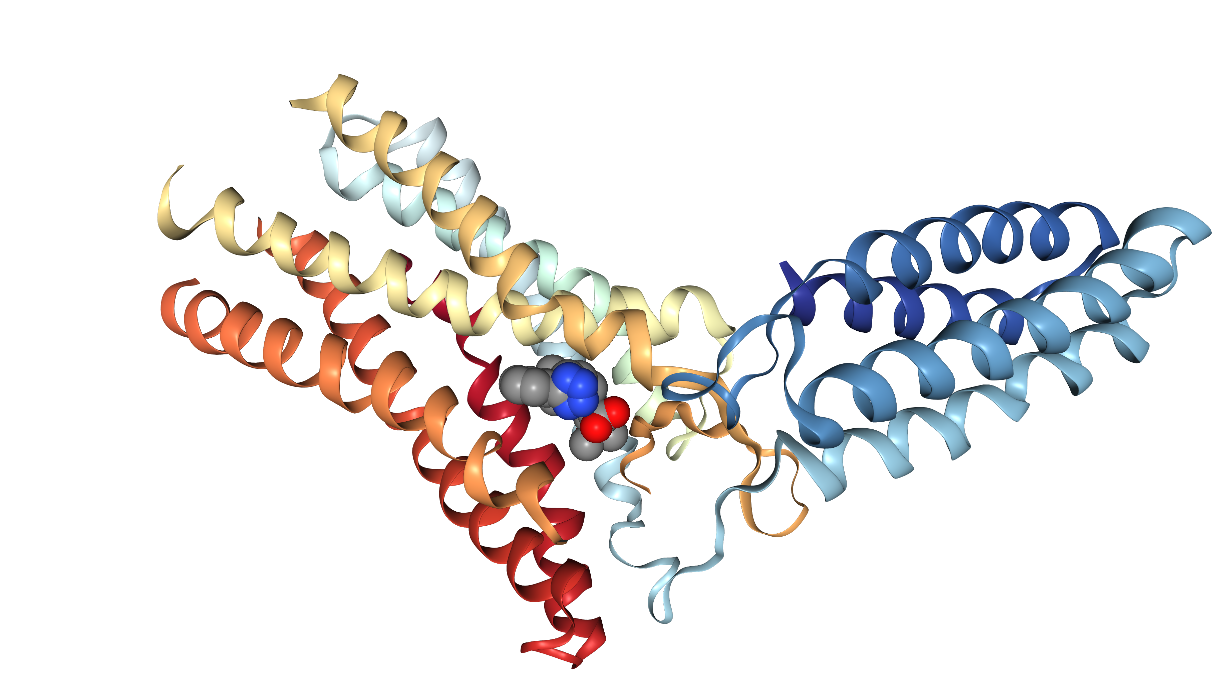
\includegraphics[width=110mm]{../pictures/4zud_screenshot}
    \end{figure}
	\small \centering Схема взаимодействия 
	лиганда-лекарства с белком-мишенью\\
	на примере структуры GPCR-рецептора AT1R с обратным агонистом олмесартаном из базы PDB.
	
\end{frame}
    
\begin{frame}{Общая картина}
	\begin{itemize}
		\normalsize
		\item Парадигма <<болезнь-мишень-лекарство>> уступает полифармакологии и лекарственной репозиции.
		\small
		\item \textit{Полифармакология}~--- одно вещество действует сразу на несколько мишеней, весь метаболический путь.\\
		$+$ меньше учет взаимодействий лекарств друг с другом;\\
		$+$ просто меньше лекарств $\rightarrow$ предсказуемость;\\
		$-$ надо создать такое лекарство.\\
		\item \textit{Лекарственная репозиция} – использование уже известных лекарств в новых целях.\\ 
		$+$ уже прошли тесты на людях $\Rightarrow$ безопасно, экономически выгодно.\\
		Примеры: виагра, некоторые лекарства от рака.
	\end{itemize}
\end{frame}

\section{Цель проекта}
\begin{frame}{Цель проекта}
	\linespread{1.35}
	\centering
    Целью работы являлось построение гибкого програмнного протокола, способного определять степени подобия лигандов/мишеней/комплексов с референсными данными, основанными на подтвержденных FDA лекарствах и протеомах.
	\small
\end{frame}

\begin{frame}{Шаги для достижения цели}	
	\begin{itemize}
		\item извлечь информацию о подтвержденных FDA лекарствах, лигандах,мишенях, а также референсных протеомах;
		\item создать функции для конвертации данных одной молекулы в требуемые сторонними программами форматы;
		\item создать функции для сравнения одного элемента входных данных с одной подтвержденной FDA записью;
		\item реализовать поиск по референсным данным наиболее подходящих в терминах различных метрик подобия для лигандов/мишеней/комплексов.
	\end{itemize}
\end{frame}
\section{Входные данные и ожидаемые результаты}
\begin{frame}{Входные данные и ожидаемые результаты}
На вход протокола могут подаваться:
\begin{enumerate}
	\item SMILES лиганда или его структура в файле SDF, MOL2, PDB;
	\item аминокислотная последовательность мишени, Uniprot ID или PDB структура;
	\item PDB структура молекулярного комплекса.
\end{enumerate}

Результат --- отсортированный по схожести ко входным данным список объектов того же типа с наиболее полной информацией о них и о различиях между входом и выходом.
\end{frame}
\section{Структура протокола}
\begin{frame}{Общая структура протокола}
\begin{figure}
	\centering
	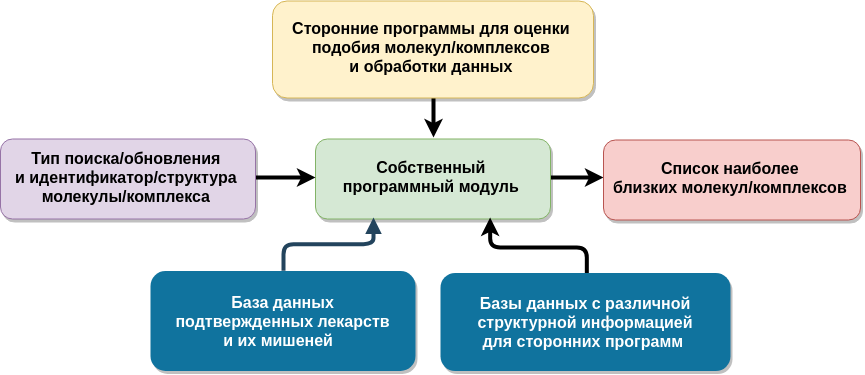
\includegraphics[width=120mm]{../Drawio/6}
\end{figure}
\end{frame}
\section{Принципы работы протокола}
\begin{frame}{Принципы работы протокола}
	Используются различные структурные метрики подобия лигандов/мишеней (последовательность, 2D-, 3D-структуры)\\
	$\:$\\
	Сайты связывания сравниваются с использованием атомистической структуры полостей в комплексах и распределения физико-химических свойств.\\
	$\:$\\
	Похожие на подтвержденные молекулы будут иметь повышенную вероятность образовать связь с теми же лигандами/мишенями и быть безвредными для человека.
	
\end{frame}

\begin{frame}{Сравнение мишеней по аминокислотной последовательности}

\end{frame}

\begin{frame}{Сравнение комплексов: нахождение полостей}
	\begin{figure}
		\centering
		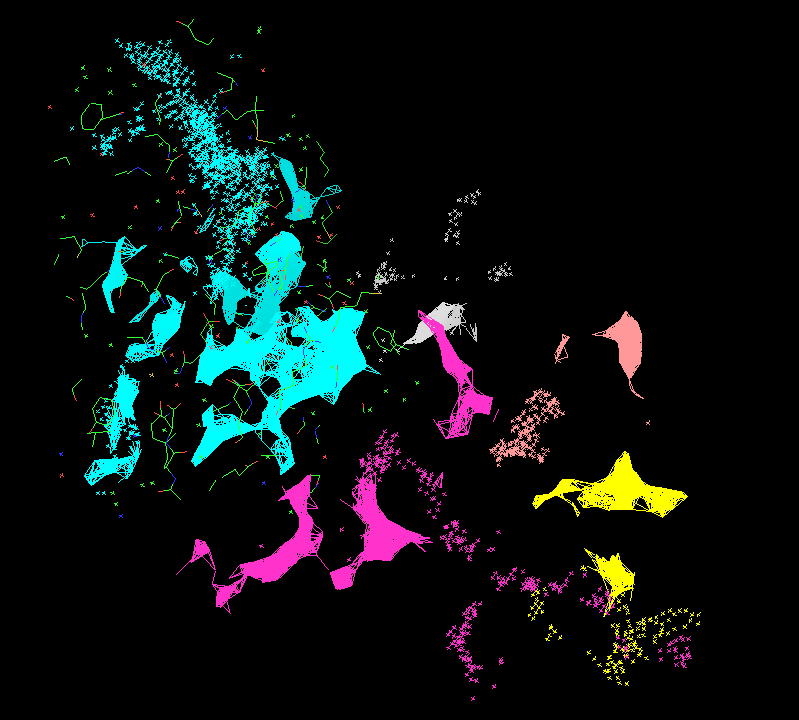
\includegraphics[width=85mm]{../pictures/clefts}		
	\end{figure}
\end{frame}

\begin{frame}{Сравнение комплексов: разметка полостей}
	\begin{figure}
		\centering
		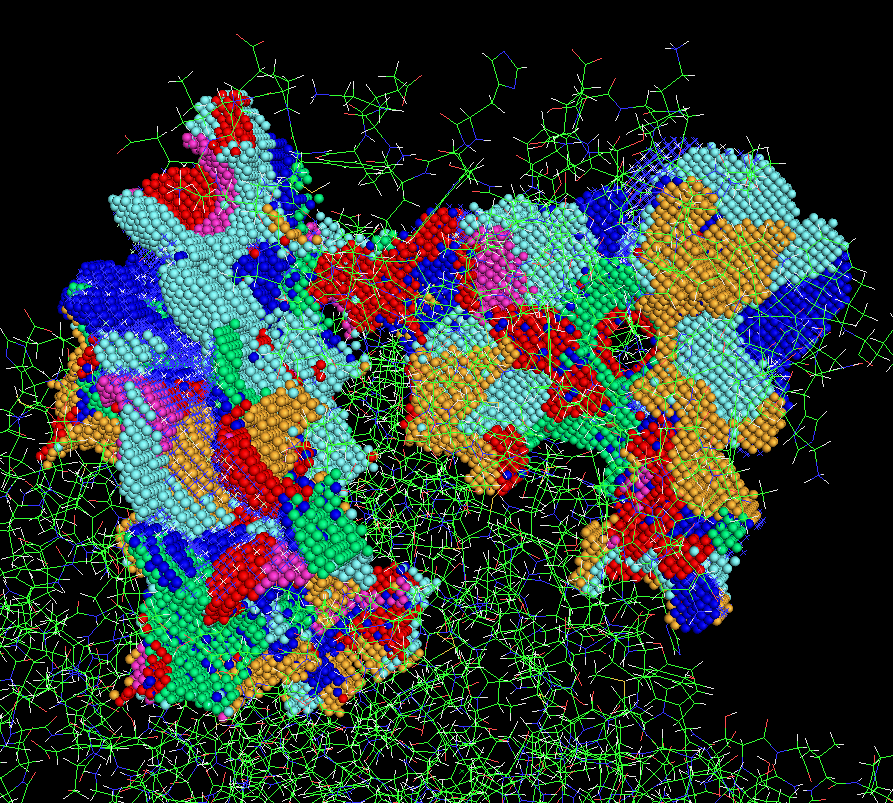
\includegraphics[width=85mm]{../pictures/mif}
\end{figure}
\end{frame}

\section{Результаты}
 \begin{frame}{Результаты}
 \end{frame}{Результаты}
 \small
 	Сравнение аминокислотных последовательностей мишеней.
     \begin{lstlisting}[label={lst:fasta}, basicstyle=\tiny]
     In:
     	get_closest_fastas_from_uniprot('P08100', path_to_data_in_fasta, k=0, align_matrix='blosum62', sim_or_ident=True)
     Out:
     
     similarity 		identity 					name
     1392 	 	1843 	348  	lcl|BSEQ0016346|Rhodopsin
     1931 	 	318 	156 	lcl|BSEQ0010278|Cholecystokinin_receptor_type_A
     151 	 	295 	147 	lcl|BSEQ0016698|Somatostatin_receptor_type_5
     ...
     Name = lcl|BSEQ0010278|Cholecystokinin_receptor_type_A
     Similarity=318.5, identity=156
     Matrix blosum62, number of alignments = 1
     MNGTEGPNFYVPFSNATGVVRSPFEYPQYY-LAEP-----WQFS---
     MLAAYMFLLIVLGFPINFLTLYVTVQHKKLRTPLNYILLNLAVADLFMVLGGFTSTLYTSLHGYFVFGPTGCNLEGFFATLGGEIAL	
     WSLVVLAIERYVVVCKPM-SNFFGENHAIMGVAFTWVMALACAAP-PLAGWSRYIP--EGLQCSCGIDYYTLKPEVNNESFVIYMFVVHFTIPMIIIFFCYGQLVFTV----------KEAAAQQQESATT------------QK---------------------------------AEKEVTRMVIIMVIAFLICWVPYA
     
     ............
     
     PISFILLLSYTSSCV--NPIIYCFMNKRFRLGFMATFPCCPNPGPPGARGEVGEEEEGGTTGASLSRFSYSHMSASVPPQ
     Score=318.5
     ...
     CPU times: user 10min 41s, sys: 1.26 s, total: 10min 42s
     Wall time: 10min 43s
     \end{lstlisting}
%\end{frame}

\section{Заключение}
\begin{frame}{Заключение}
	
\end{frame}

\end{document}


%------------------------------------------------

\begin{frame}
\frametitle{Multiple Columns}
\begin{columns}[c] % The "c" option specifies centered vertical alignment while the "t" option is used for top vertical alignment

\column{.45\textwidth} % Left column and width
\textbf{Heading}
\begin{enumerate}
\item Statement
\item Explanation
\item Example
\end{enumerate}

\column{.5\textwidth} % Right column and width
Lorem ipsum dolor sit amet, consectetur adipiscing elit. Integer lectus nisl, ultricies in feugiat rutrum, porttitor sit amet augue. Aliquam ut tortor mauris. Sed volutpat ante purus, quis accumsan dolor.


\section{Заключение}
\begin{frame}{Cactus Graph}
	\begin{itemize}
		\item Definition: A graph in which any two vertices are at most two-edge connected
		\item Each edge is apart of at most one simple cycle
		\item Suppose we have a graph G which is not a cactus graph. 
		\item We can create a mapping from $G \rightarrow G'$; a graph homomorphism that maps each vertex in set $V_G$ into $V_G'$
		\item The set of vertices mapped to in $G'$ is 2 edge connected 
	\end{itemize}
\end{frame}

%------------------------------------------------
\section{Заключение}
%------------------------------------------------

\begin{frame}
\frametitle{Table}
\begin{table}
\begin{tabular}{l l l}
\toprule
\textbf{Treatments} & \textbf{Response 1} & \textbf{Response 2}\\
\midrule
Treatment 1 & 0.0003262 & 0.562 \\
Treatment 2 & 0.0015681 & 0.910 \\
Treatment 3 & 0.0009271 & 0.296 \\
\bottomrule
\end{tabular}
\caption{Table caption}
\end{table}
\end{frame}

%------------------------------------------------


\begin{frame}
\frametitle{References}
\footnotesize{
\begin{thebibliography}{99} % Beamer does not support BibTeX so references must be inserted manually as below
\bibitem[Smith, 2012]{p1} John Smith (2012)
\newblock Title of the publication
\newblock \emph{Journal Name} 12(3), 45 -- 678.
\end{thebibliography}
}
\end{frame}

%------------------------------------------------

\begin{frame}
\Huge{\centerline{The End}}
\end{frame}

%----------------------------------------------------